In \textbf{Unsupervised Learning}, $\mathcal{D}$ contains no labels.\\
Models both define labels \& assign inputs to labels.
$$
    \mathcal{D} = \Bigl\{ x_1,\ldots,x_n \Bigr\}    \qquad      \text{\color{gray}\footnotesize(Dataset in unsupervised learning)}
$$
There are many use-cases:
\begin{enumerate}
    \item Compression
    \item Discovery of latent variables
    \item Anomaly detection
    \item Exploratory data analysis
\end{enumerate}

\subsection{Clustering}

\definition \textbf{Clustering}

The goal here is to group inputs into clusters, based on some definiton of similarity, e.g. $l_2$ distance for $\mathcal{D} \subset \R^2$.\\
\subtext{This can be seen as the unsupervised analogy to classification}

\subsubsection{Basic Methods}

\method \textbf{Hierarchical Clustering}

A simple method, using the "similarity" measure directly.

\begin{enumerate}
    \item Each $x \in \mathcal{D}$ starts in its own cluster
    \item Iteratively, the $2$ "closest" clusters are merged
\end{enumerate}

This results in a tree, thus \textit{hierarchical} clustering.

\method \textbf{Partitioning}

In Partitioning methods, a weighted graph is constucted using $\mathcal{D}$ and partitioned using graph theory approaches, i.e. using cuts or spectral analysis.

{\footnotesize
    \remark Both Hierarchical and Partitioning do not give a natural way to deduce cluster membership for new datapoints.
}

\newpage

\subsubsection{$k$-Means Clustering}

In $k$-means, a cluster is represented by its center: $\mu_j \in \R^d$.
The cluster assignment $z_i$ for $x_i \in \mathcal{D}$:
$$
    z_i = \underset{j=1,\ldots,k}{\text{arg min}}\Bigl\Vert x_i-\mu_j \Bigr\Vert    \qquad {\color{gray}\footnotesize \text{(Closest center)} }
$$
{\footnotesize
    \remark This strategy induces a partition of $\R^d$. (Voronoi Pattern)
}

\textbf{Problem}: How to find $\mu = (\mu_1,\ldots,\mu_k)^\top$?

A new optimization objective:
$$
    \hat{R}(\mu) = \sum_{i=1}^n \underset{j\in\{1,\ldots,k\}}{\min}\Bigl\Vert x_i-\mu_j \Bigr\Vert^2 = \sum_{i=1}^n \Bigl\Vert x_i-\mu_{z_i} \Bigr\Vert
$$
\subtext{(minimize the sum of sq. distances between points \& their centers)}

{\footnotesize
    \remark $\Vert\cdot\Vert_2$ corresponds to the \textit{mean}. $\Vert\cdot\Vert_1$ would use the \textit{median}.
}

So we are searching: (non-convex \& NP-hard)
$$
    \underset{\mu}{\text{arg min}} \Bigl( \hat{R}(\mu) \Bigr) \qquad {\color{gray}\footnotesize \text{(optimal $k$-means cluster)}}
$$

\method \textbf{Lloyd's Heuristic}

This is an iterative method to find the cluster centers.

{\footnotesize
    \definition $z^{(t)} = \Bigl( z_1^{(t)},\ldots,z_n^{(t)} \Bigr)^\top$ \color{gray}(assignment of $x_i$ at iter. $t$)\color{black}

    \definition $\mu^{(t)} = \Bigl( \mu_1^{(t)},\ldots,\mu_k^{(t)}\Bigr)^\top$ \color{gray}(Cluster centers at iter. $t$)\color{black}

    \definition $n_j^{(t)} = \Bigl| \Bigl\{ i=1,\ldots,n\ \Big|\ z_j^{(t)}=j \Bigr\} \Bigr|$ \color{gray}(Size of cluster $j$ at iter. $t$)\color{black}
}

\begin{algorithm}
    \caption{Lloyd's Heuristic}
    $\mu^{(0)}\gets \Bigl( \mu_1^{(0)},\ldots,\mu_k^{(0)} \Bigr)$\;
    \SetKwRepeat{Do}{repeat}{until}
        \Do{\text{convergence}}{ 
            $z_i^{(t)} \gets \underset{j \in \{1,\ldots,k\}}{\text{arg min}}\Bigl\Vert x_i-\mu_j^{(t-1)} \Bigr\Vert\quad\ $ for $i=1,\ldots,n$ \;
            $\mu_j^{(t)} \gets \frac{1}{n_j^{(t)}}\displaystyle\sum_{i \text{ s.t. } z_{i}^{(t)}=j} x_i\qquad\qquad$ for $j=1,\ldots,k$ \;
            $t \gets t+1$ \;
        }
\end{algorithm}
{\footnotesize
    \remark Each iteration is in $\mathcal{O}\bigl( nkd \bigr)$.
}

% Continue with convergence analysis, k-means++

\subsubsection{Convergence}

$k$-Means is guaranteed to converge to a local optimum:

\theorem \textbf{Motonically decreasing convergence}\\
\smalltext{$\forall t \geq 1:$}
$$
    \hat{R}\bigl( \mu^{(t)},z^{(t)} \bigr) \geq \hat{R}\bigl( \mu^{(t+1)},z^{(t+1)} \bigr)
$$

{\footnotesize
    \remark For the global optimum, the initialization is critical.
}

{\footnotesize
    \remark $k$-Means may produce bad results for non-sperical clusters.\\ 
    \color{gray}(A consequence of using $\Vert\cdot\Vert_2$, kernels can overcome this)
}

\subsubsection{initialization}

\textbf{Problem}: How to choose $\mu^{(0)} = \Bigl(\mu^{(0)}_1,\ldots,\mu^{(0)}_k  \Bigr)$?

\textbf{Solution}: Heuristics.

A simple approach is sampling uniformly from $\mathcal{D} = \{x_1,\ldots,x_n\}$. However, This is problematic for unbalanced cluster sizes.\\
\subtext{The chance that small clusters receive no initial $\mu^{(0)}_i$ is high.}

\method \textbf{Furthest Point Heuristic}\\
Select $\mu^{(0)}_0$ randomly, then iteratively maximize distance to the nearest cluster center for subsequent $\mu^{(0)}_{i\geq1}$.

\method \textbf{k-means++}\\
More robust heuristic: more random factors against outliers.

\textbf{Step 1}: Pick $\mu^{(0)}_0$ randomly.
$$
    \mu^{(0)}_0 = x_i \in \mathcal{D}, \qquad i \sim \mathcal{U}\bigl(\{1,\ldots,n\}\bigr)
$$
\textbf{Step 2}: Pick $\mu^{(0)}_{2,\ldots,k}$ using this rule.
$$
    \mu^{(0)}_j = x_i \in \mathcal{D}, \qquad i \sim p(i) \propto \underset{1 \leq m \leq j-1}{\min}\bigl\Vert x-\mu_m \bigr\Vert^2
$$

\theorem \textbf{k-means++ is optimal up to} $\mathcal{O}\bigl(\log(k)\bigr)$
$$
    \hat{R}\bigl( \mu_\text{k-means++} \bigr) \leq \mathcal{O}\bigl(\log(k)\bigr)\cdot \underset{\mu}{\min} \hat{R}(\mu)
$$

\subsubsection{Choosing $k$}

\textbf{Problem}: How to choose $k$?

{\footnotesize
    \remark Unfortunately, cross-validation can't be used: Both the training \& test loss will decrease as $k$ increases, so the loss provides no good stopping criterion.
}

\method Increase $k$ until $\hat{R}$ yields diminishing returns.\\
\subtext{Usually, plotting $k$ against $\hat{R}$ yields something like $\exp$ decay.}
% Lecture 29.04: Nonlinear k-means/PCA with kernels, NOT in script

\method Penalize higher model complexity.\\
\subtext{weight $\lambda > 0$ is generally easier to choose than $k$ directly.}
$$
    \hat{R}' = \hat{R}(\mu) + \lambda\cdot k
$$

There are several other methods to do this, based e.g. on concepts from information theory.

\newpage

\subsection{Principal Component Analysis}

\textbf{Motivation}: For $\mathcal D = \{x_i\}_{i=1}^n,x_i\in\R^d$, we'd like a low-dimentional representation with $k \ll d$, which we call \textit{embeddings} $\{z_i\}_{i=1}^n, z_i\in\R^k$.\\
\subtext{e.g. for performance, memory, noise removal, visualizations...}

{\footnotesize
    \textbf{Intuition}: High dimensional data usually has many redundancies \& highly correlated features. Dimensionality Reduction in practice preserves most substantial data. This idea is formalized as the \textit{Manifold Hypothesis}.

    \remark \textbf{Requirement}: We assume $\mathbf{X}$ is centered. For general $\mathbf{X}$, we therefore use:
    $$
        \bar{\mathbf{X}} = \mathbf{X} - \mathbf{I}\mu \qquad \mu = \sum_{i=1}^{n}x_i
    $$
    i.e. we subtract the mean $\mu$ of all $x_i$ from each $x_i$.
}

\subsubsection{PCA in one dimension}

\method \textbf{PCA $k=1$}\\
\smalltext{Find $w^*\in\R^d$ and $z_1^*,\ldots,z_2^*\in\R$ for dimensionality reduction $d=1$:}
$$
    w^*,z_1^*,\ldots,z_n^* = \underset{w\in\R^d : \Vert w\Vert_2 = 1}{\min}\sum_{i=1}^{n}\underbrace{\Bigl\Vert x_i-\overbrace{z_iw}^{\approx x} \Bigr\Vert}_\text{Reconstruction Error}
$$

\begin{center}
    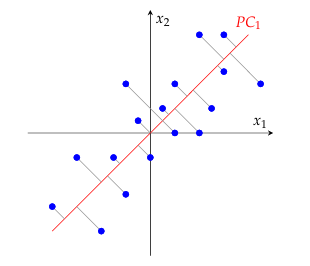
\includegraphics[width=0.35\linewidth]{resources/pca1d.png}\\
    \subtext{Introduction to Machine Learning (2026), p. 223}
\end{center}

\lemma \textbf{PCA $k=1$ (Variance Matrix)}\\
\smalltext{Alternative formulation.}
$$
    w^* = \underset{\Vert w \Vert_2=1}{\text{arg max}}\ w^\top \Sigma w
$$

{\footnotesize
    \textbf{Intuition}: $w$ can be thought of as the subspace (a line for $d=1$) we want to project onto. The optimal $w^*$ aligns with the direction maximizing the \textit{empirical variance} $\Sigma$ of the projected data.
}

\definition \textbf{Empirical Covariance} $\displaystyle\Sigma = \frac{1}{n}\sum_{i=1}^{n}x_ix_i^\top = \frac{1}{n}X^\top X$

\lemma \textbf{Eigendecomposition} $\displaystyle\Sigma = \sum_{i=1}^{d}\lambda_iv_iv_i^\top$\\
\subtext{Eigenvalues $\lambda_1 > \ldots > \lambda_d > 0$,\\ 
eigenvectors $v_i$ forming an orthonormal Basis of $\R^d$}

\theorem \textbf{PCA Solution for $k=1$}\\
\smalltext{$v$ is the Eigenvector associated with the largest $\lambda$ for $\Sigma$.}
$$
    w^* = v_1 \quad \text{solves} \quad w^* = \underset{\Vert w \Vert_2=1}{\text{arg max}}\ w^\top \Sigma w
$$

\subsubsection{Generalized PCA}

Luckily, the case $k=1$ generalizes:

\theorem \textbf{PCA General Solution}\\
\smalltext{Here, $\mathbf{W}\in\R^{d\times k}$ and $z_i^* \in \R^k$ for parameter $k$}
$$
    \mathbf{W}^*,z_1^*,\ldots,z_n^* = \underset{\mathbf{W}\in\R^{d\times k}: \mathbf{W}^\top\mathbf{W}=\mathbf{I}}{\text{arg min}} \sum_{i=1}^{n} \Bigl\Vert x_i - \mathbf{W}z_i \Bigr\Vert^2
$$
is solved using
$$
    \mathbf{W}^* = \Bigl( v_1 \| \cdots \| v_k \Bigr), \qquad z_i^* = \mathbf{W}^{*\top}x_i
$$

{\footnotesize
    \textbf{Intuition}: In words, the basis for the $k$-dim. subspace minimizing reconstruction error is given using the first $k$ eigenvectors of $\Sigma$.
}

\lemma \textbf{PCA is an orthohgonal projection} 
$$
    P: \R^d\to\R^d,\qquad x \mapsto \mathbf{W}^*\mathbf{W}^*x
$$

\lemma \textbf{Connection to SVD}\\
\smalltext{The First $k$ EV of $\Sigma$ are the first $k$ right singular vectors of $\mathbf{X}$.}
$$
    \mathbf{X} = \mathbf{USV}^\top \qquad n\cdot\Sigma = \mathbf{VS}^\top \mathbf{SV}^\top
$$

{\footnotesize
    \remark Non-linear methods and kernels can be applied to PCA the same way they are applied to regression.
}

\newpage 
\subsubsection{Connection to k-Means}

k-Means (Clustering) can be reformulated: $z_1,\ldots,z_n \in E_k$ where $E_k = \{e_1,\ldots,e_n\}$ holds unit vectors $e_i$.
$$
    \mathbf{W}^*,z_1^*,\ldots,z_n^* = \underset{\mathbf{W}\in\R^{d\times k}: \mathbf{W}^\top\mathbf{W}=\mathbf{I}}{\text{arg min}} \sum_{i=1}^{n} \Bigl\Vert x_i - \mathbf{W}z_i \Bigr\Vert^2
$$
This is the same as PCA, only the space for $z^*$ changes. Both PCA and k-Means are special forms of a more general technique:

\definition \textbf{Matrix Factorization Methods}\\
\smalltext{General class of techniques for decomp. of $\mathbf{X}$}
$$
    \mathbf{X} \approx \mathbf{WZ}
$$

{\footnotesize
    \remark \textbf{PCA}. For PCA, $\mathbf{W}$ is an orthonormal Basis of the optimal $k$-dimenional subspace, $\mathbf{Z}$ are the coefficients for the projection.

    \remark \textbf{k-Means}. For k-means, $\mathbf{W}$ contains cluster centroids and $\mathbf{Z}$ the cluster assignments.
}
